% 3. Data Corpus and Preprocessing Methodology
\section{The Need for Unification}
\label{ch:data_methodology}

This section presents an overview of the need for a unified framework for trajectory prediction in autonomous driving, addressing the challenges of dataset heterogeneity and the complexities of motion forecasting tasks. The discussion highlights the importance of standardizing data formats, feature characteristics, and preprocessing pipelines to enable effective model training and evaluation across diverse datasets.

\subsection{Unification of Motion Forecasting Datasets}
\label{sec:data_datasets}

The \texttt{UniTraj} framework addresses the fundamental challenge of standardizing multiple motion-forecasting datasets that exhibit substantial heterogeneities in both \emph{data formats} and \emph{feature characteristics}.
The former encompasses differences in data structure and organization, while the latter stems from variations in
spatio-temporal resolution, coverage range, and semantic annotation schemes.

To overcome format discrepancies, \texttt{UniTraj} leverages \texttt{ScenarioNet}~\cite{scenarionetLi2023} for conversion into a common
format, thereby eliminating the need for multiple preprocessing implementations. However, feature characteristics require additional harmonization. Temporal coverage varies substantially
across datasets, with historical trajectories ranging from 1 second in \texttt{WOMD}\cite{wmodSun2020} to 5 seconds in \texttt{Argoverse 2}\cite{av2Wilson2023},
and future prediction horizons extending from 6 to 8 seconds. Map resolutions and semantic annotations differ
significantly, with all datasets providing \emph{scene-centric} HD maps at varying resolutions.
Agent features also exhibit substantial variations: \texttt{nuScenes} provides only velocity and heading, while
\texttt{WOMD} includes comprehensive 3D bounding box annotations. Notably, \texttt{Argoverse 2} provides bounding
box and rich semantic annotations, but these are lost during \texttt{ScenarioNet} format conversion.
The normalization of the feature spaces is performed through a multi-stage processing, and its results are outlined in~\autoref{app:framework}.


% The UniTraj framework integrates three major autonomous driving datasets: Argoverse2 (AV2)~\cite{av2Wilson2023}, NuScenes~\cite{caesar2020nuscenes}, and Waymo Open Dataset~\cite{wmodSun2020}. Each dataset contributes unique characteristics:

% \begin{itemize}
%     \item \textbf{Argoverse2:} High-resolution HD maps with detailed lane topology, focusing on highway and urban scenarios
%     \item \textbf{NuScenes:} Multi-modal sensor data with 360° coverage, diverse weather and lighting conditions
%     \item \textbf{Waymo:} Large-scale dataset with consistent labeling and comprehensive scene coverage
% \end{itemize}

% The amalgamation strategy standardizes coordinate systems, temporal sampling rates, and feature representations across datasets~\cite{VectorNet2020, Shi2022MTR}. This unified approach enables cross-dataset training and evaluation while preserving dataset-specific characteristics through metadata annotations.

% The fusion methodology addresses inherent dataset heterogeneities through a nine-phase preprocessing pipeline (detailed in Appendix~\ref{app:notation}) that transforms raw data into consistent \texttt{DatasetItem} representations. This approach follows established practices in trajectory prediction literature~\cite{zhou2022hivt, qcnetZhou2023, Shi2023MTRplusplus}.

% \subsection{Remaining ML Infrastructure}
% This subsection outlines the need for further essential components required to develop motion forecasting models, and why it would be beneficial to unify them in a single framework such that the research communicty can focus on the model architecture and training, rather than the implementation details of the infrastructure.
% This includes logging and experiment tracking, distributed training, configuration management, evaluation metrics, visualization tools




\subsection{Limitations of UniTraj}
\label{sec:data_challenges}

Implementation of the unified framework revealed significant challenges affecting data quality and model generalizability, aligning with known issues in autonomous driving dataset integration.

When creating unified dataset, given multiple source datasets, they did not respect the original train, val, and test splits which is a common practice in machine learning

None of the most important sym

\subsection{Data Integration and Representational Limitations}
\label{ssec:data_limitations}

Critical limitations emerged during dataset integration, reflecting broader challenges in autonomous driving data standardization~\cite{hu2023planning}. Dataset heterogeneity manifests through inconsistent feature availability: Agent type availability varies inconsistently—while Waymo provides comprehensive pedestrian and cyclist annotations, Argoverse2 focuses primarily on vehicle trajectories, creating domain-specific biases~\cite{unitrajFeng2024}.\\
Temporal and spatial standardization introduces information loss, highlighting trade-offs between unification and data fidelity. Varying sampling rates (10Hz vs 20Hz) require interpolation that potentially loses behavioral nuances. Feature quantization for computational efficiency reduces predictive accuracy, while fixed scene radii exclude relevant distant objects affecting long-range interactions.

\subsection{Framework Implementation Issues and Mitigation Strategies}
\label{ssec:framework_issues}

The original UniTraj implementation suffered from critical software quality deficiencies that significantly impacted model performance and generalization across domains~\cite{metadriveLi2022}. The most significant limitation was the absence of PyTorch Lightning integration, forcing manual implementation of training infrastructure that modern ML frameworks provide standardized~\cite{falcon2019pytorch}. Additional problems included poor code organization with tight coupling between components, lack of modular design patterns, and insufficient testing frameworks, making the system difficult to maintain, extend, or debug effectively.
The training infrastructure lacked essential deep learning capabilities: automatic mixed precision training, gradient accumulation, learning rate scheduling, and distributed computing support. Manual implementation of these features resulted in suboptimal performance, excessive memory usage, and limited scalability. The framework also lacked integrated experiment tracking with tools like Weights \& Biases or TensorBoard, hampering reproducibility and systematic model development workflows.
Mitigation strategies follow modern ML engineering best practices, with PyTorch Lightning migration as the primary solution. This architectural change provides structured training loops, automatic optimization, distributed computing support, and seamless experiment tracking integration~\cite{falcon2019pytorch}. Additional improvements include codebase refactoring into modular components, comprehensive unit and integration testing implementation, continuous integration adoption, and enhanced logging capabilities through Lightning's callback system for better visibility into training dynamics across datasets~\cite{unitrajFeng2024, scenarionetLi2023}.


\subsubsection{Revision of the UniTraj Framework}
This section details the major modifications we applied to the original UniTraj framework to achieve a more modular, type-safe, and production-ready codebase.

\paragraph{Data handling and preprocessing refinements.}
\begin{itemize}[leftmargin=*]
  \item \textbf{Strongly typed interfaces:} Introduced \href{https://github.com/JanDuchscherer104/UniTraj/blob/main/unitraj/datasets/types.py}{\texttt{types.py}} to declare all input and output tensors via \texttt{TypedDict} and dataclasses, replacing untyped \texttt{dict} passes and surfacing shape mismatches at static analysis time. Defines \texttt{RawScenarioDict}, \texttt{ProcessedDataDict} and other interfaces.
  \item \textbf{Decoupled parsing pipeline:} Split the monolithic script into three stages—\href{https://github.com/JanDuchscherer104/UniTraj/blob/main/unitraj/datasets/base_dataparser.py}{\texttt{base\_dataparser.py}} (handles raw file ingestion and basic conversions), \href{https://github.com/JanDuchscherer104/UniTraj/blob/main/unitraj/datasets/dataparser.py}{\texttt{dataparser.py}} (implements the nine-phase QC preprocessing pipeline), and \href{https://github.com/JanDuchscherer104/UniTraj/blob/main/unitraj/datasets/base_dataset.py}{\texttt{base\_dataset.py}} (wraps processed data into a PyTorch \texttt{Dataset} class), enabling modular parser swaps without code changes.
  \item \textbf{PyTorch Lightning integration:} Built a \href{https://github.com/JanDuchscherer104/UniTraj/blob/main/unitraj/lightning/lit_datamodule.py}{\texttt{lit\_datamodule.py}} (defines \texttt{LightningDataModule}) and \href{https://github.com/JanDuchscherer104/UniTraj/blob/main/unitraj/lightning/lit_trainer_factory.py}{\texttt{lit\_trainer\_factory.py}} (instantiates \texttt{pl.Trainer} from config) to configure \texttt{pl.Trainer} via YAML, unlocking multi-GPU, mixed-precision, and gradient accumulation with <30LoC of overhead and removing ~300LoC of boilerplate.
  \item \textbf{Full Weights \& Biases (WandB) support:} Added \href{https://github.com/JanDuchscherer104/UniTraj/blob/main/unitraj/configs/wandb_config.py}{\texttt{wandb\_config.py}} (configures WandB logger and callbacks) and Lightning callbacks to log hyperparameters, metrics, and checkpoint artefacts directly to WandB, replacing ad-hoc CSV dumps and enabling real-time dashboards.
\end{itemize}

\paragraph{Architecture Overview}
The revised UniTraj framework follows a hierarchical configuration-driven architecture that enables modular component instantiation and type-safe data flow. Figure~\ref{fig:unitraj_data_architecture} illustrates the core data handling components and their relationships within the framework.

\begin{figure}[htbp]
    \centering
    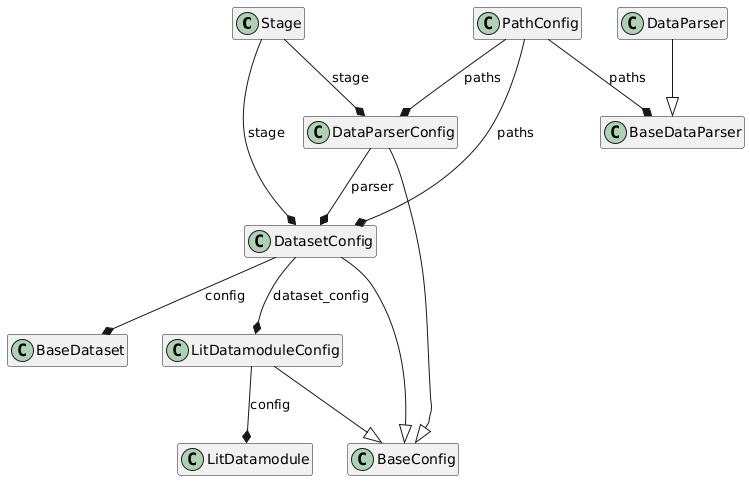
\includegraphics[width=0.9\textwidth]{figures/classes_DataHandling.png}
    \caption{UniTraj data handling architecture showing the relationships between configuration classes, data parsers, datasets, and Lightning modules. The diagram illustrates the Config-as-Factory pattern implementation and the modular data processing pipeline.}
    \label{fig:unitraj_data_architecture}
\end{figure}

The architecture comprises four primary layers:

\begin{itemize}[leftmargin=*]
    \item \textbf{Configuration Layer:} The \texttt{BaseConfig} class serves as the foundation for all configuration objects, implementing the Config-as-Factory pattern through the \texttt{setup\_target()} method. The \texttt{PathConfig} centralizes all filesystem paths and is automatically propagated to child configurations during instantiation. The \texttt{Stage} enum defines dataset splits (train/validation/test) and ensures consistent stage handling across the pipeline.
    \item \textbf{Data Processing Layer:} The \texttt{BaseDataParser} provides the interface for raw data ingestion, while \texttt{DataParser} implements the nine-phase preprocessing pipeline that transforms ScenarioNet format into normalized feature representations. The \texttt{DataParserConfig} controls preprocessing behavior including multiprocessing settings, cache management, and debug mode configuration.
    \item \textbf{Dataset Layer:} The \texttt{BaseDataset} wraps processed data into PyTorch-compatible format, implementing efficient data loading with optional H5PY file handles for large-scale datasets. The \texttt{DatasetConfig} manages dataset instantiation parameters and integrates the parser configuration for end-to-end data pipeline control.
    \item \textbf{Lightning Integration Layer:} The \texttt{LitDatamodule} provides PyTorch Lightning-compatible data loading with automatic train/validation/test split handling, configurable batch sizes, and multiprocessing support. The \texttt{LitDatamoduleConfig} enables declarative dataloader configuration from YAML files while maintaining type safety through Pydantic validation.
\end{itemize}

The composition relationships shown in the diagram reflect the framework's dependency injection approach: configurations contain references to their dependencies rather than hard-coded instantiations, enabling flexible component swapping and comprehensive testing. For instance, the \texttt{DatasetConfig} contains both a \texttt{DataParserConfig} and stage information, allowing different parsing strategies per dataset split without code duplication.

\paragraph{Configuration and path management.}
\begin{itemize}[leftmargin=*]
  \item \textbf{Config-as-Factory pattern:} Implemented \href{https://github.com/JanDuchscherer104/UniTraj/blob/main/unitraj/utils/base_config.py}{\texttt{base\_config.py}} (defines \texttt{BaseConfig} and \texttt{setup\_target()}) methods, allowing declarative instantiation of datasets, trainers, and models from YAML/JSON without touching code.
  \item \textbf{Centralized PathConfig:} Consolidated all filesystem paths (data root, logs, checkpoints) in \href{https://github.com/JanDuchscherer104/UniTraj/blob/main/unitraj/configs/path_config.py}{\texttt{path\_config.py}} (centralizes filesystem paths) and ensured automatic directory creation, eliminating scattered \texttt{os.makedirs()} calls.
  \item \textbf{Experiment reproducibility:} Integrated hierarchical overrides and \href{https://github.com/JanDuchscherer104/UniTraj/blob/main/unitraj/utils/base_config.py}{\texttt{base\_config.py}} (provides \texttt{inspect()} for config trees) to print the full resolved config tree at startup, improving traceability of parameter sweeps.
\end{itemize}

\paragraph{General refactoring and model zoo expansion.}
\begin{itemize}[leftmargin=*]
  \item \textbf{Modular model registry:} Refactored the \texttt{models/} folder into sub-packages (e.g., \texttt{autobot}, \texttt{mtr}, \texttt{wayformer}), each with its own \href{https://github.com/JanDuchscherer104/UniTraj/blob/main/unitraj/models/base_model/base_model.py}{\texttt{base\_model.py}} (defines \texttt{BaseModel} and \texttt{BaseModelConfig}), standardizing the interface for adding new architectures.
  \item \textbf{Utility consolidation:} Moved logging, console output, and visualization routines into \href{https://github.com/JanDuchscherer104/UniTraj/blob/main/unitraj/utils/console.py}{\texttt{console.py}} (provides structured \texttt{Console} API) modules, replacing ad-hoc print statements with a structured \texttt{Console} API.
  \item \textbf{Typed function signatures:} Audited all \texttt{.py} files to add precise type annotations for inputs and outputs (e.g., \texttt{batch: list[DatasetItem] -> BatchDict}), enabling \texttt{mypy} enforcement and catching runtime errors early.
\end{itemize}

\newpage